\chapter{Background}
\label{background}
Learning is one of the most interesting functions of the human mind. If we think of the human memory as a storage of beliefs, we may think of learning as the manipulation of these beliefs. In that sense, learning something new would correspond to the addition of new beliefs. But learning is not only about new things. We sometimes learn things that contradict other things we learned before. In that sense, learning could be thought of as the update or revision of beliefs. 

In this chapter, we aim at explaining the context of the ideas developed in this study, and giving some background of the main building blocks of our work. We will discuss three different ways of changing beliefs and we will use the AGM framework\cite{kr} to define and explain these changes. After explaining the AGM rules that govern our approaches to rational belief change, we will explain a Description Logic called $\mathcal{EL}$, which will be used in this study as the knowledge representation language.

\section{Belief change}
The AGM framework is named after Alchourron, Gardenfors, and Makinson, the three scientists who invented it in the 1980s. Since that time, AGM has been the most adopted framework for belief change. In \cite{flux}, Gardenfors came up with some very useful notations to describe the change of beliefs, \textit{epistemic states} and \textit{attitudes}. We can think of the epistemic states as the states of mind (from the beliefs perspective), where epistemic states of an agent are defined by the epistemic attitudes agents have towards the concepts they know about. In this case, changing one attitude towards one concept implies a new epistemic state. Therefore, belief change is simply transitions between different epistemic states. Before moving on to explaining the AGM paradigm, it is useful to shed some light on the notions of epistemic states and attitudes.

\subsection{Epistemic states}
As the word ``change" suggests, our concern is about transitions between epistemic states. One can think of an epistemic state as the state of beliefs of an agent (or a human), and of the change as the move from a given state to a new state. The beliefs of an agent can be modelled -as the epistemological theory suggested in \cite{flux}- as a set of propositions (or beliefs), with some assumptions on the attitudes towards each of the propositions (will be discussed in more details in \ref{epistemicAttitudes}.) Those beliefs are not meant to be psychological propositions expressing beliefs in human mind; they are epistemological \textit{idealizations} of psychological propositions that a human mind can believe or reject. It is reasonable to consider that every agent should always seek an \textit{equilibrium} state, where the epistemic state is consistent; and if some concepts are contradicting, the agent ought to revise its beliefs to reach a consistent state. 

In this study, we use the words ``belief sets" and ``epistemic state", and they are not exactly the same, although they are related; A \textbf{Belief Set} is the set of all things that an agent believe in, while an \textbf{Epistemic State} is the complete state of the agent's epistemic attitudes towards all propositions, including the ones that the agent does not believe in. Depending on the epistemological model we follow, we might consider propositions that are not in the belief set to be rejected, or we might assume that the agent neither believes in them nor rejects them. 

Another important notion is the \textit{belief base}, which we use to refer to the (possibly incomplete) set of \textit{explicit} beliefs of an agent. It is different from a belief set because we typically assume that belief sets are closed under logical consequence, while belief bases are not. In that sense, we say that the belief set includes some \textit{implicit} beliefs that follow from some explicit ones.

The AGM paradigm will use the notion of belief sets. Later in \ref{dl}, we will discuss Description Logics (DLs) as formalisms to express knowledge, and start using DL \textit{concepts} to represent belief bases. All following discussions about \textit{contraction} algorithms will use such representation.


\subsection{Epistemic attitudes}
\label{epistemicAttitudes}
A belief of an agent can be interpreted according to the concepts in an epistemic state. Suppose the concept $C$ is defined as:
\begin{center}
$C$ = It's Monday
\end{center}
If $C$ exists in the belief set of an agent, we say that the agent believes in $C$ (believes that today is Monday), or \textit{accepts} $C$ \cite{flux}, which also means that accepting $C$ is part of the epistemic state of the agent. However, \textit{accepting} a belief is not the only attitude an agent can have towards a concept. An agent can also \textit{reject} a concept $C$ if the negation of that concept is in the belief set (i.e. It is not Monday.) In that epistemic state, we say that the agent rejects $C$. It is also possible that an agent stays \textit{undetermined} (or ignorant) about a concept if neither the concept nor its negation is in the belief set (e.g. an agent has no idea whether today is Monday or not.) There can be more attitudes if we consider other models of beliefs such as the probabilistic model, where an agent might have different levels of beliefs. But for the scope of this study we are only interested in the three attitudes: \textit{accept}, \textit{reject} and \textit{no clue}.

\subsection{Basic types of change}
The AGM framework defines three types of belief change: \textit{revision}, \textit{expansion}, and \textit{contraction}. If one sees a flying penguin, it introduces a new belief (penguins might fly), which contradicts another belief people these days have: penguins can't fly. In this case, just accepting the new belief will make the belief system of the agent (In this case, a human) inconsistent, since two beliefs are contradicting. So revising the old beliefs, and possibly removing the belief about penguins can't fly, is the rational action humans tend to take. This is referred to as belief revision.

When we add a new belief without removing old beliefs, we call this process \textit{belief expansion}. When a belief is removed, or given up, without accepting a new belief, we call this process \textit{belief contraction}. A good example of belief contraction is to give up a belief for the sake of argument, to reach a common ground with an opponent, and argue based on this ground.

Before going further into details of those types of change of belief, some important notions need to be explained.

\begin{description}
\item[belief set]

We represent the beliefs of an agent by a set of sentences, where $\{A\}$ represents a belief set of only one belief $A$. So an agent who has $\{A\}$ as his belief set only believes in $A$, and is ignorant everything else. The belief set is closed under deductive inference; if $K$ is a belief set, then $K \vdash \alpha$ if and only if $\alpha \in K$.
\end{description}

Given a belief set $K$ and a sentence $A$, we say $K \vdash A$ if and only if A is a consequence of the belief set $K$. We refer to the set of all consequences of $K$ by $Cn(K)$. Since $K$ is a belief set, then it is closed under deduction. Hence, $K = Cn(K)$, where $Cn(K)$ is the deductive closure of $K$. For any belief set $K$ and a sentence $A$, we can represent the three aforementioned epistemic attitudes as follows \cite{flux}:

\begin{itemize}
\item If $A \in K$, $A$ is \textit{accepted} and $-A$ is \textit{rejected}.

\item If $-A \in K$, $A$ is \textit{rejected}, and $-A$ is \textit{accepted}.

\item $A \notin K$ and $-A \notin K$ means that $A$ is \textit{undetermined}.
\end{itemize}

We can think of belief change about $A$ as a change of the attitude towards $A$. Because we have three attitudes, we have six possible changes. However, because of the symmetry of some pairs of change we only consider three types of change:

\begin{enumerate}
\item Change from being \textit{undetermined} to either \textit{accepting} or \textit{rejecting} $A$ (can only be obtained through \textit{expansion}).
\item Change from \textit{accepting} to \textit{rejecting} and vice versa (\textit{revision}).
\item Change from \textit{accepting} or \textit{rejecting} $A$ to being \textit{undetermined} (\textit{contraction})\cite{flux}.
\end{enumerate}

\subsubsection{Belief Expansion}
As part of the learning process and gaining knowledge an agent expands its belief set by \textit{accepting} new beliefs. If $K$ is a belief set and $A$ is a statement, then $K^{+}_{A}$ is the new belief set resulting from accepting $A$. So the expansion function $+$ is a function that takes a belief set $K$ and a statement $A$ and returns another belief set $K^{+}_{A}$. 

\subsubsection{Belief Contraction}
Contraction is different from expansion. Expansion by $A$ is the change from the state of not accepting nor rejecting it to the state of accepting it, while contraction is the change from accepting or rejecting $A$ to being undetermined of it. We denote the belief set resulting from contracting the belief set $K$ with respect to sentence $A$ by $K^{-}_{A}$. Since contraction is the most relevant change to the scope of this study, we need to discuss some of the rationality criteria (or postulates) of such change. We consider the contraction function $-$ as a function from a set of beliefs $K$ and a sentence $A$ to a new set of beliefs $K^{-}_{A}$ as in \cite{flux} and \cite{kr}. 

In the AGM framework, the following eight postulates ((K $-$ 1) to (K $-$ 8)) are introduced as basis for ensuring the rationality of contraction functions (more details can be found in \cite{kr} and \cite{flux}):


\begin{description}
\item[(K $-$ 1)] For any sentence $A$ and any belief set $K$, $K^{-}_{A}$ is a belief set.
\end{description}
$K^{-}_{A}$ is obtained by removing some beliefs. So
\begin{description}
\item[(K $-$ 2)] $K^{-}_{A} \subseteq K$. 
\end{description}
If $A$ is not already in the belief set, the contraction should not change the belief set.
\begin{description}
\item[(K $-$ 3)] If $A \notin K$, then $K^{-}_{A} = K$. 
\end{description}
Unless $A$ is logically valid, $A$ should not be in the belief set after contraction.
\begin{description}
\item[(K $-$ 4)] If not $\vdash A$, then $A \notin K^{-}_{A}$. 
\end{description}


The main idea of contraction is to give up some belief (maybe temporarily). If we need to give $B$ up we can remove it from the belief set, and make sure it is not derivable from the remaining beliefs. To do that we need to look for statements that together entail $B$ and remove at least one of them. This will be elaborated more in chapter \ref{kernel} when we discuss kernels. So we do not just remove $A$ from $K$, but remove the minimum number of sentences that would entail $A$. We remove the ``minimum" number of sentences because it is better to give up as least as possible (minimum change will be explained in more details in chapter \ref{kernel}). Also, while performing expansion with $A$ we compute all possible consequences that can be reached after accepting $A$. Therefore, all beliefs are recoverable by expansion after contraction:
\begin{description}
\item[(K $-$ 5)] If $A \in K$, then $K \subseteq (K^{-}_{A})^{+}_{A}$.
\end{description}
If $A$ and $B$ are equivalent sentences, then contracting $K$ for the belief $A$ should result in the same belief set as contracting it for $B$.
\begin{description}
\item[(K $-$ 6)] If $\vdash A \leftrightarrow B$, then $K^{-}_{A} = K^{-}_{B}$.
\end{description}
If we contract $K$ by $A \& B$, we should contract $K$ by either $A$ or $B$, but nothing else.
\begin{description}
\item[(K $-$ 7)] $K^{-}_{A} \cap K^{-}_{B} \subseteq K^{-}_{A \& B}$.
\end{description}
Motivated by the concept of minimal change, the last postulate states that if $A$ was removed while contracting $K$ by $A \& B$, then at least $A$ was given up -- possibly along with $B$.
\begin{description}
\item[(K $-$ 8)] If $A \notin K^{-}_{A \& B}$, then $K^{-}_{A \& B} \subseteq K^{-}_{A}$.
\end{description}

These eight postulates (K $-$ 1) -- (K $-$ 8) assume that contraction of belief sets. However, in this study we are investigating the contraction of belief bases. 

In \cite{hansson}, Hansson declared that an operator for $A$ is a kernel contraction (kernels will be explained later) if and only if it satisfies the postulates of \textit{success}, \textit{inclusion}, \textit{core-retainment}, and \textit{uniformity}. We are discussing these postulates because they are more applicable in our investigation of kernel contraction. They are explained in \cite{hansson} as follows (the symbol $\div$ denotes contraction, e.g. $K^{-}_{A}$ is equivalent to $K \div A$):

\begin{description}
\item[Success] If $\alpha \notin Cn(\emptyset)$, then $\alpha \notin Cn(A \div \alpha)$.
\end{description}
This is similar to \textbf{(K $-$ 4)}.

\begin{description}
\item[Inclusion] $A \div \alpha \subseteq A$.
\end{description}
This is similar to \textbf{(K $-$ 2)}.

\begin{description}
\item[Core-retainment] If $\beta \in A$ and $\beta \notin A \div \alpha$, then there is a set $A'$ such that $A' \subseteq A$ and that $\alpha \notin Cn(A')$ but $\alpha \in Cn(A' \cup \{ \beta \})$.
\end{description}
This implies that only sentences that contribute to making $A$ imply $\alpha$ can be removed during contraction, and nothing else. 

\begin{description}
\item[Uniformity] If it holds for all subsets $A'$ of $A$ that $\alpha \in Cn(A')$ if and only if $\beta \in Cn(A')$, then $A \div \alpha = A \div \beta$.
\end{description}
This is similar to \textbf{(K $-$ 6)}.

\subsubsection{Belief Revision}
Revision is different from expansion and contraction, as it is considered to be \textit{non-monotonic}. New beliefs are added with -possibly- some of the old beliefs removed. Revision takes place when the attitude is changed from accepting to rejecting or from rejecting to accepting. We can think of revision as a combination of both contraction and expansion. The revision function $*$ is a function from a belief set $K$ and a sentence $A$ to a belief set $K^{*}_{A}$. If $-A \in K$, then $K^{*}_{A} = (K^{-}_{-A})^{+}_{A}$.

In the next section we look at a class of languages called Description Logic that is being used these days to represent knowledge. We use it as a model and implement contraction in a DL-based knowledge bases.


\section{Description logic}
\label{dl}
One of the earliest approaches to representing knowledge is using logic. Logic has been suitable for general-purpose applications. Another approach is what is so-called semantic networks, which is a graph (or a network)-based approach. Semantic networks use graphs to represent knowledge\cite{dl}, where nodes represent \textit{concepts} and edges represent \textit{relationships} between them.

\textit{Description Logic} (DL) comes as an evolution of semantic networks to a logic-based approach with some new flavours. DL is a class of logics based on -as the name suggests- describing sets of individuals using \textit{concepts} and describing the relationships between them using \textit{roles}. Usually, two types of knowledge need to be represented: \textit{intensional} and \textit{extensional} knowledge. Intensional knowledge is general knowledge about a problem or a domain, while extensional knowledge is knowledge about a specific problem instance. For this purpose, a knowledge base\footnote{By the word \textit{Knowledge base} we refer to a belief base -- a set of sentences that represent the belief of an agent.} is composed of two main components: Terminological Box, which we will refer to by \textit{TBox}, and Assertions Box, which we refer to by \textit{ABox}.

To get an idea about what DL looks like, we look at two categories of symbols: logical and non-logical symbols. \textbf{Non-logical} symbols include the following:
\begin{description}
\item[Concepts] that are similar to category nouns (e.g. $Human$, $Mother$, $Animal$, $College$, etc.). They are used to represent classes (or sets) of individuals. So we can use the concept $Animal$ to refer to the set of animals, and the concept $Man$ to represent the class of men.
\item[Roles] that are like relational nouns (e.g. $MotherOf$, $HeightOf$, etc.). They can be used to specify attributes of concepts.
\item[Constants] and they are used to represent individuals, and they are similar to proper nouns, e.g. $Adam$, $Sally$, etc.
\end{description}

Concepts and roles can be used with the help of some logical symbols to construct complex expressions. \textbf{Logical} symbols include the following:
\begin{itemize}
\item $\sqcap, \sqcup, \neg$ used as propositional constructors (conjunction, disjunction, and negation respectively).
\item $\forall, \exists$ used for restriction and quantification.
\item $\top, \bot$ ($\top$ represents the set of all individuals, while $\bot$ represents the empty set of individuals). 
\end{itemize}

Logical and non-logical symbols can be used together to construct complex expressions. To get a sense of how to build complex expressions, suppose $C$ and $D$ are concepts, and $R$ is a role:
\begin{itemize}
\item $C \sqcap D$, $C \sqcup D$, and $\neg C$ are concepts (also called concept expressions).
\item $\forall R.C$, and $\exists R.\top C$ are concepts (or concept expressions).
\end{itemize}


\subsection{ABox}
As we said at the beginning of this section, to represent knowledge we usually look at intensional and extensional knowledge. DL knowledge bases usually consist of two main components: TBox and ABox. \textbf{ABoxes} are built from assertions (extensional knowledge) about a specific problem or domain, e.g.
\begin{center}
$Girl(Sally)$ may represent the fact that $Sally$ is a $Girl$ and, \\
$FatherOf(Adam, Sally)$ may represent the fact that $Adam$ is the $Father$ $Of$ $Sally$
\end{center} 
where $Sally$ and $Adam$ are constants, $Girl$ is a concept name, and $FatherOf$ is a role name. Using such representation, ABoxes can be built to represent assertions about a problem or a domain.


\subsection{TBox}
Suppose that $Human$ is a concept that refers to all humans, and $Male$ is the concept that refer to all male beings. We can use conjunction ($\sqcap$) in
\begin{center}
$Human \sqcap Male$
\end{center}
to represent all individuals that are both humans and male beings. We can also define a new concepts $Man$ to represent those individuals by introducing the definition
\begin{center}
$Man \doteq Human \sqcap Male$
\end{center}
So every man has to satisfy that definition. The $TBox$ is composed of concept definitions and General Concept Inclusion rules (GCIs). GCIs are weaker than definitions; the rule
\begin{center}
$Man \sqsubseteq Human$
\end{center}
states that $Man$ is subsumed by $Human$, which means that every man is a human\footnote{or more precisely, every member of the set represented by $Man$ is also a member of the set represented by $Human$.}. Every definition can be safely broken down into two GCIs. For example, the definition
\begin{center}
$Man \doteq Human \sqcap Male$
\end{center}
can be broken down into the two GCIs:
\begin{center}
$Man \sqsubseteq Human \sqcap Male$ \\
$Human \sqcap Male \sqsubseteq Man$
\end{center}

\textbf{Tboxes} are used to represent general knowledge (intensional knowledge) about a class of problems or domains, using axioms (or terminologies). A typical TBox is composed of definitions and GCIs -- sometimes for convenience all definitions are broken down into GCIs. The following is an example of a -somewhat incomplete- DL TBox:
\begin{enumerate}
\item $Man \doteq Human \sqcap Male$.
\item $Woman \sqsubseteq Human \sqcap \neg Man$.
\item $Father \doteq Man \sqcap \exists ParentOf. \top$
\item $Mother \doteq Woman \sqcap \exists ParentOf. \top$
\item $FatherWithoutSon \doteq Father \sqcap \forall ParentOf. \neg Man$.
\item $Parent \doteq Father \sqcup Mother$
\item $GrandFather \sqsubseteq Father \sqcap \exists ParentOf.Parent$
\end{enumerate}
where they can be interpreted such that \#1 defines $Man$ to be a human male, \#2 states that every $Woman$ is a human and not a man, \#3 defines $Father$ to be a man that is a parent of something (since $\top$ includes everything), \#4 defines $Mother$ similarly, \#5 defines a $FatherWithoutSon$ to be a father which every individual that is in a ``$ParentOf$" relationship with is not a man, \#6 defines a $Parent$ to be a father or a mother, and \#7 states that every $GrandFather$ is a father and in a ``$ParentOf$" relation ship with a parent.

Along with some other symbols and constructors, these symbols are the building blocks of DL formalisms. There are many members of the DL family, that vary in their expressivity power and the complexity of their reasoning algorithms. Each member of the family includes a subset of the DL symbols, and is uniquely identified by the containment of those symbols. In the following section we discuss a very famous member of the DL family, $\mathcal{EL}$, and use it as a knowledge representation language for the rest of the study.


\subsection{$\mathcal{EL}$ language}
One of the DLs that recently became famous and attracted much attention is $\mathcal{EL}$. $\mathcal{EL}$ is a light-weight Description Logic, though it is used in some well-known ontologies such as SNOMED CT, which is a medical ontology that contains around 380000 concepts\cite{new}. $\mathcal{EL}$ only contains a subset of the concept constructors that we discussed in the previous section, and they are:
\begin{itemize}
\item The conjunction symbol $\sqcap$
\item Existential restriction $\exists$
\item The top concept $\top$
\end{itemize}

One of the advantages of $\mathcal{EL}$, besides being simple and easy to use, is its polynomial-time subsumption algorithm. The subsumption problem, which is the most important problem in $\mathcal{EL}$, is actually a classification problem. The subsumption algorithm classifies the $TBox$ depending on the subsumption relation expressed by $\sqsubseteq$. It is basically checking whether a specific subsumption relation holds or not (e.g. whether $C \sqsubseteq D$ holds or not) in a given knowledge base. Checking whether a subsumption relation holds or not is also checking whether the concept (or concept expression) on the left-hand side of the subsumption relation is subsumed by the concept on the right-hand side.

It is helpful to sketch the subsumption algorithm before moving on into the core of this study, as it will be used later on. But we will use an example to see how the algorithm can be applied. Let's assume we have a knowledge base TBox $\mathcal{T}$ that consists of only two subsumption relations:
\begin{center}
$\mathcal{T}$ = $\lbrace$ Haddock $\sqsubseteq$ Fish, Fish $\sqsubseteq$ Animal. $\rbrace$
\end{center}
The first one states that every Haddock is a Fish, and the second one states that every Fish is an Animal. Now, given that $\mathcal{T}$, we need to check that every Haddock is an Animal:
\begin{center}
Haddock $\sqsubseteq$ Animal.
\end{center}
This is not explicitly stated in $\mathcal{T}$, but we can imply it using the subsumption algorithm. The algorithm proceeds in four steps:
\begin{enumerate}
\item Normalize the TBox.
\item Translate the normalized TBox into a graph.
\item Complete the graph using completion rules.
\item Read off the subsumption relationships from the normalized graph.
\end{enumerate}
We can follow the four steps and apply them one by one to our example and get the solution that we need.
\subsubsection{Normalize the TBox}
We can only call a TBox normalized if all the GCIs it contains are of any of the following forms:
\begin{itemize}
\item $A_1 \sqcap A_2 \sqsubseteq B$
\item $A \sqsubseteq \exists r.B$
\item $\exists r.A \sqsubseteq B$
\end{itemize}
where $A$, $A_1$, $A_2$, and $B$ are concept names, and $r$ is a role name. A TBox can be normalized in polynomial time. $A \sqcap \top$ is equivalent to $A$. So, the normalized version of the $\mathcal{T}$ look like:
\begin{center}
$\lbrace$ Haddock $\sqcap$ $\top$ $\sqsubseteq$ Fish, Fish $\sqcap$ $\top$ $\sqsubseteq$ Animal $\rbrace$.
\end{center}

\subsubsection{Translate the normalized TBox into graph}
The second step is to translate the TBox into a graph. This is done by creating a node that corresponds to each concept in the TBox (including $\top$), and have an edge between every pair of nodes. We use $S$ to denote the set of nodes' labels, and $R$ to denote the set of roles' labels. $S$ will contain the subsumers of a node, e.g. $S(A)$ contains $B$ if $A$ $\sqsubseteq$ $B$. Likewise, $R(A, B)$ contains $r$ if $A$ $\sqsubseteq$ $\exists r.B$. Initially, the set $S$ starts by containing the nodes and $\top$, i.e. $S(Haddock)= \lbrace Haddock, \top \rbrace$, $S(Fish) = \lbrace Fish, \top \rbrace$, and $S(Animal)= \lbrace Animal , \top \rbrace$. The set $R$ will initially be empty. The graph can be visualised in Figure \ref{hdk}. Translating the TBox into a graph can be done in polynomial time.

\begin{figure}
\centering
\fbox{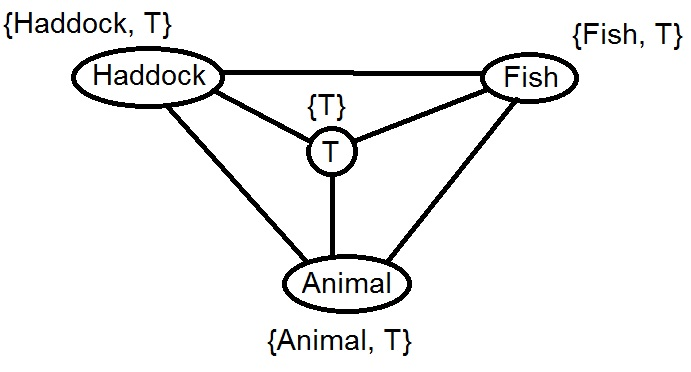
\includegraphics[scale=0.5]{Haddock-graph-with-T.jpg}}
\caption{Graph transformation of the TBox}
\label{hdk}
\end{figure}

\subsubsection{Complete the graph using completion rules}
The following three rules are then used to extend the sets $S$ and $R$:
\begin{itemize}
\item If $(A_1 \sqcap A_2 \sqsubseteq B) \in \mathcal{T}$ and $A_1, A_2 \in S(A)$ then add $B$ to $S(A)$
\item If $(A_1 \sqsubseteq \exists r.B) \in \mathcal{T}$ and $A_1 \in S(A)$ then add $r$ to $R(A, B)$
\item If $(\exists r.B_1 \sqsubseteq A_1) \in \mathcal{T}$ and $B_1 \in S(B), r \in S(A, B)$ then add $A_1$ to $S(A)$ 
\end{itemize}
If we apply the completion rules to $\mathcal{T}$, $S$ will become as follows:
\begin{itemize}
\item $S(Animal)= \lbrace Animal, \top \rbrace$
\item $S(Fish)= \lbrace Fish, \top, Animal \rbrace$
\item $S(Haddock) = \lbrace Haddock, \top, Fish, Animal \rbrace$
\end{itemize}
The new graph (after the completion rules are applied) can be visualised in Figure \ref{hdk-complete}. 

\begin{figure}
\centering
\fbox{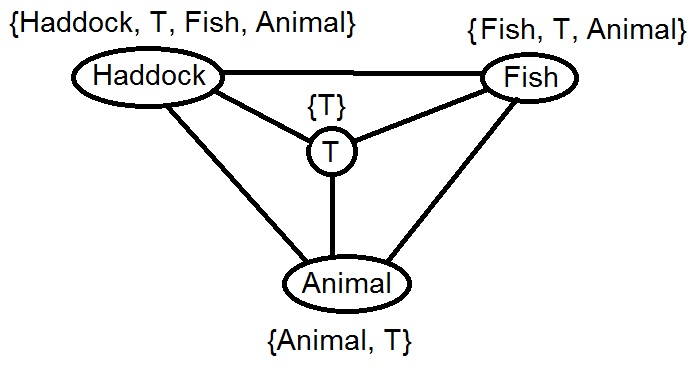
\includegraphics[scale=0.5]{Haddock-graph-with-T-complete.jpg}}
\caption{Completed graph of the TBox}
\label{hdk-complete}
\end{figure}

\subsubsection{Read off the subsumption relationships}
Now that the graph is complete, we can look at the sets $S$ and $R$ and determine whether the subsumption relationship in question holds or not. Since that subsumption relationship was $Haddock \sqsubseteq Animal$, we can look at $S(Haddock)$ and see if it contains $Animal$ or not, since the set $S(Haddock)$ contains all subsumers of $Haddock$. So, indeed, $Haddock \sqsubseteq Animal$ holds. This brief example hopefully shows a simple application of the subsumption algorithm of $\mathcal{EL}$. We didn't discuss the complexity of the algorithm in details, but it is enough to say it is polynomial in the size of the TBox. More details on the algorithm can be found in \cite{small} and \cite{new}.

Now that we had a quick introduction to the basic types of belief change and the framework of AGM, as well as the $\mathcal{EL}$ language and reasoning algorithm, we can start talking about the core of this study, which is kernel contraction. Throughout this study, we only consider DL knowledge bases represented in $\mathcal{EL}$. In the next chapter we look at an implementation of belief contraction using \textit{kernels} as introduced in \cite{zwei}. We will discuss some basic and general approaches as well as some more sophisticated ones. Then we will consider a language-specific approach to exploit the structure of $\mathcal{EL}$ and discuss heuristics that will provide more meaningful solutions. 